\begin{frame}[shrink=5]{Hydrostatic equations for ice sheet flow}
  \begin{itemize}
  \item Valid when $w_x \ll u_z$, independent of basal friction {\small (Schoof\&Hindmarsh 2010)}
  \item Eliminate $p$ and $w$ from Stokes by incompressibility:\\
    \quad 3D elliptic system for $\bm u = (u,v)$
    \begin{align*}
      - \nabla\cdot \left[ \eta
        \begin{pmatrix}
          4 u_x + 2 v_y & u_y + v_x & u_z \\
          u_y + v_x & 2 u_x + 4 v_y & v_z
        \end{pmatrix} \right] + \rho g \bar\nabla h & = 0
    \end{align*}
    \begin{align*}
      \eta(\theta,\gamma) &= \frac{B(\theta)}{2} (\gamma_0 + \gamma)^{\frac{1-\mathfrak n}{2\mathfrak n}}, \qquad \mathfrak n \approx 3 \\
      \gamma &= u_x^2 + v_y^2 + u_xv_y + \frac 1 4 (u_y+v_x)^2 + \frac 1 4 u_z^2 + \frac 1 4 v_z^2
    \end{align*}
    and slip boundary $\sigma \cdot \bm n = \beta^2 \bm u$ where
    \begin{align*}
      \beta^2(\gamma_b) &= \beta_0^2 (\epsilon_b^2 + \gamma_b)^{\frac{\mathfrak m-1}{2}}, \qquad 0 < \mathfrak m \le 1 \\
      \gamma_b &= \frac 1 2 (u^2 + v^2)
    \end{align*}
  \item $Q_1$ FEM with Newton-Krylov-Multigrid solver in PETSc: \code{src/snes/examples/tutorials/ex48.c}
  \end{itemize}
\end{frame}

\frame{
  \vspace{-8em}
  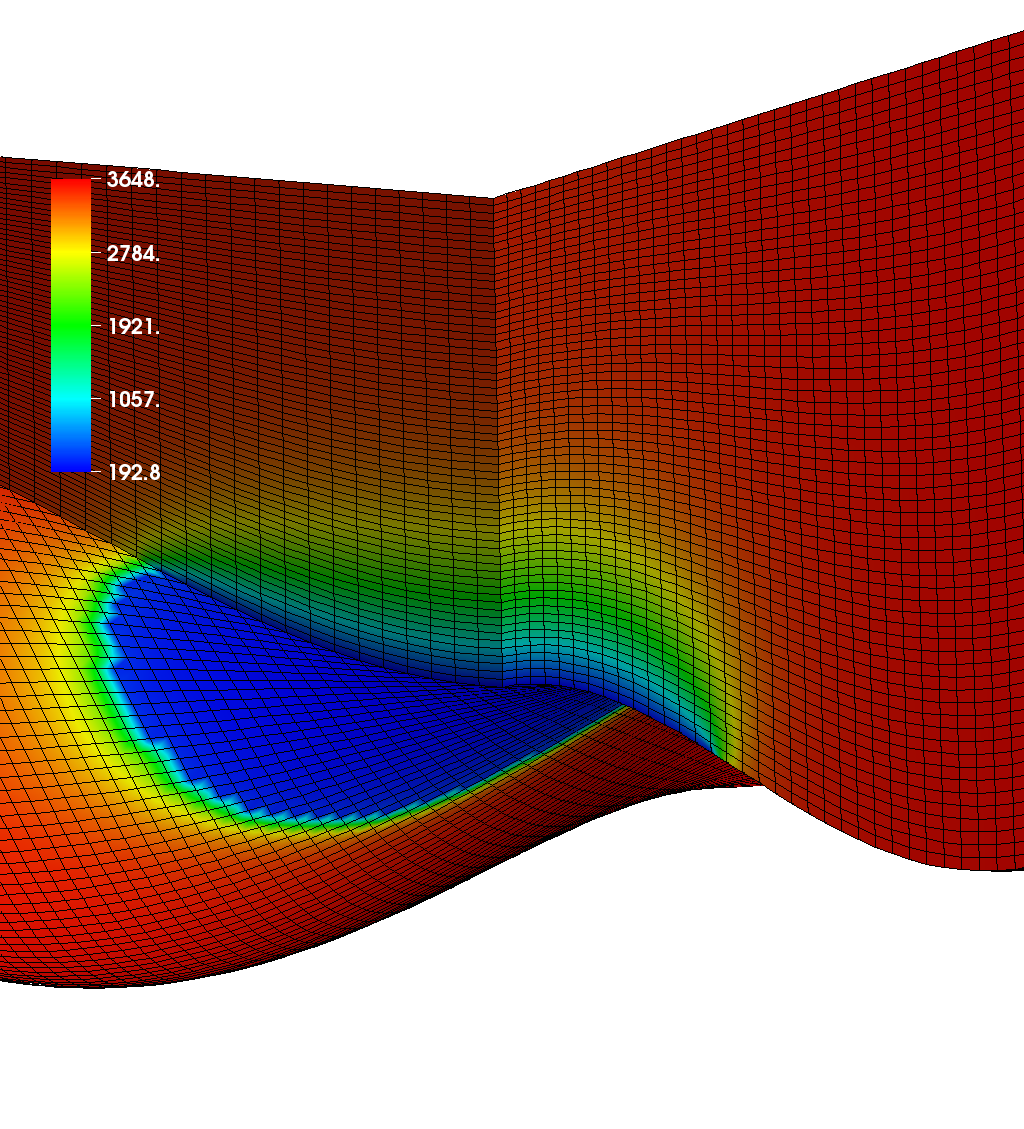
\includegraphics[width=1.2\textwidth]{figures/THI/x-5km-m8p5l5-clip}
}


\begin{frame}{Some Multigrid Options}
  \begin{itemize}
  \item \code{-dmmg\_grid\_sequencce}: [FALSE] \\
    Solve nonlinear problems on coarse grids to get initial guess
  \item \code{-pc\_mg\_galerkin}: [FALSE] \\
    Use Galerkin process to compute coarser operators
  \item \code{-pc\_mg\_type}: [FULL] \\
    (choose one of) MULTIPLICATIVE ADDITIVE FULL KASKADE
  \item \code{-mg\_coarse\_\{ksp,pc\}\_*} \\
    control the coarse-level solver
  \item \code{-mg\_levels\_\{ksp,pc\}\_*} \\
    control the smoothers on levels
  \item \code{-mg\_levels\_3\_\{ksp,pc\}\_*} \\
    control the smoother on specific level
  \item These also work with ML's algebraic multigrid.
  \end{itemize}
\end{frame}

\begin{frame}{What is this doing?}
\begin{itemize}
\item
\begin{alltt}\footnotesize
mpiexec -n 4 ./ex48
-M 16
-P 2
-da\_refine\_hierarchy\_x 1,8,8 \\
-da\_refine\_hierarchy\_y 2,1,1
-da\_refine\_hierarchy\_z 2,1,1 \\
-dmmg\_grid\_sequence 1
-dmmg\_view
-log\_summary \\
-ksp\_converged\_reason
-ksp\_gmres\_modifiedgramschmidt \\
-ksp\_monitor
-ksp\_rtol 1e-2 \\
-pc\_mg\_type multiplicative \\
-mg\_coarse\_pc\_type lu
-mg\_levels\_0\_pc\_type lu \\
-mg\_coarse\_pc\_factor\_mat\_solver\_package mumps \\
-mg\_levels\_0\_pc\_factor\_mat\_solver\_package mumps \\
-mg\_levels\_1\_sub\_pc\_type cholesky \\
-snes\_converged\_reason
-snes\_monitor
-snes\_stol 1e-12 \\
-thi\_L 80e3
-thi\_alpha 0.05
-thi\_friction\_m 0.3 \\
-thi\_hom x
-thi\_nlevels 4
\end{alltt}
\item What happens if you remove \code{-dmmg\_grid\_sequence}?
\item What about solving with block Jacobi, ASM, or algebraic multigrid?
\end{itemize}
\end{frame}
